\section{Solving the multi-objective WSN problem}
\label{section:solution}
As defined in the previous Section, we seek a method to optimise multiple objectives in our WSN system. To do so we will incorporate two algorithms. Firstly, the \acronymATARIAExtended{}{} algorithm will enable agents in the system to learn the best agents to allocate tasks to to obtain the best composite task values, as well as explore the system for other agents, and adapt to impacts and outages. The second, the \acronymMGRAOExtended{}{} algorithm, helps agents executing measurement tasks allocate their resources to optimise the composite task value as well.


%%%%%%%%%%%%%%%%%%%%%%%
\newcommand{\formalATARIA}[2]{
	\functionFormal{ataria}
	{XXX}
	{\powerSetAgents{}{} \times \powerSetAgents{}{} \times (\setAction{}{} \times \setRealNumbers{}{})}
}
%%%%%%%%%%%%%%%%%%%%%%%%%

\subsection{Optimising for task allocation with system exploration}
\todo[inline]{Summary of ATARIA algorithm, connected to our problem notation, why we use it and the outcome}

\subsection{Resource allocation in agents taking measurements}
\todo[inline]{Summary of MGRAO algorithm, connected to our problem notation, why we use it and the outcome}

\subsection{Extension to hierarchical task allocation}

XXXX

\todo[inline]{Integrated view of the algorithms plus a flow diagram for illustration}

\begin{figure}
	\centering
	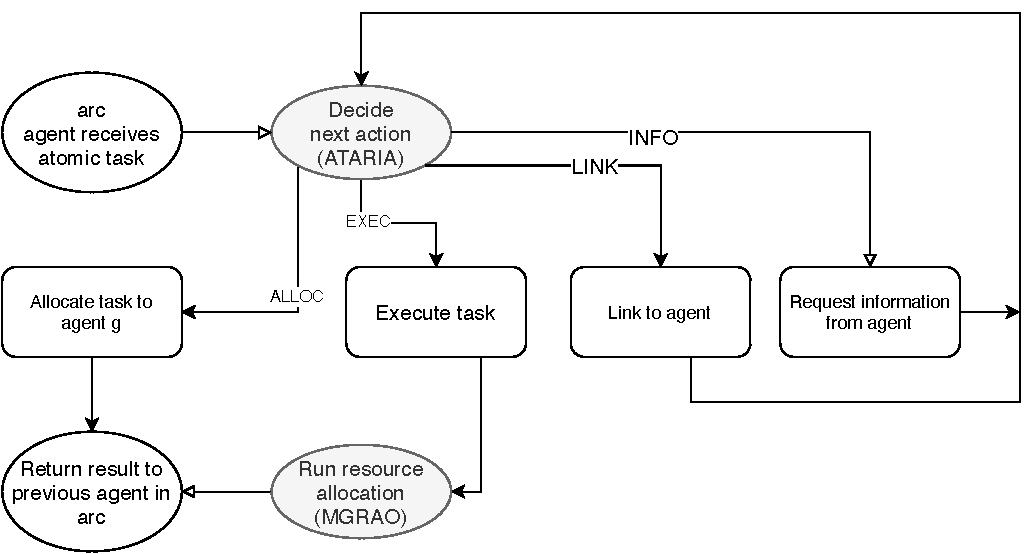
\includegraphics[width=0.9\linewidth]{algorithm-flow}
	\caption{\textbf{Flow chart of combined \acronymATARIA{}{}/\acronymMGRAO{}{} execution}. The two algorithms are combined together to allow recursive allocation of tasks and learning of the network}
	\label{fig:algorithm-flow}
\end{figure}
\begin{figure}
	\centering
	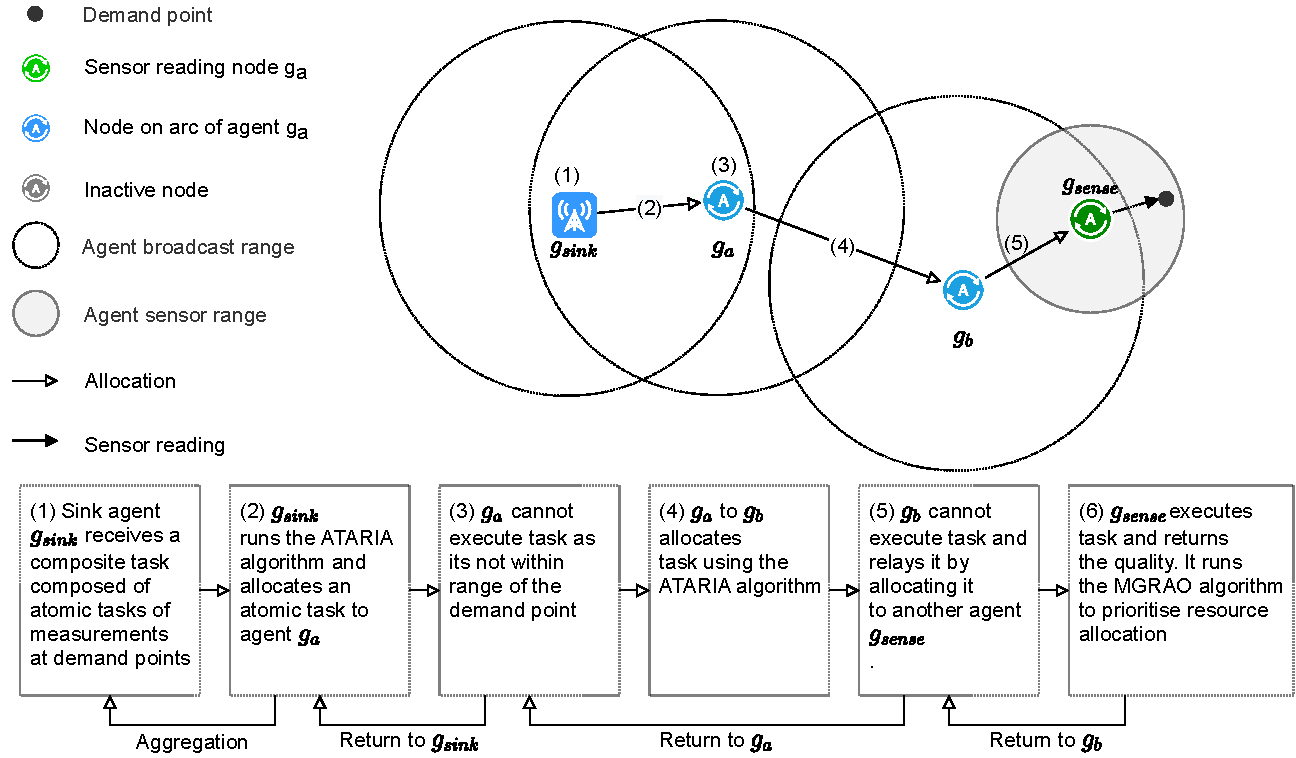
\includegraphics[width=0.9\linewidth]{arc-flow}
	\caption{\textbf{Allocation along an arc}. This diagram illustrates how allocations can be relayed along an arc using successive applications of the \acronymATARIA{}{} algorithm.}
	\label{fig:arc-flow}
\end{figure}